
%DIF LATEXDIFF DIFFERENCE FILE
%DIF DEL ..\Summary_v1\Summary_flat.tex   Wed Mar 13 15:13:38 2024
%DIF ADD Summary_flat.tex                 Wed Mar 13 15:13:35 2024

\documentclass[a4paper, 10pt, conference, oneside]{ieeeconf}      

\overrideIEEEmargins
\usepackage{geometry}
 \geometry{
 a4paper,
 total={170mm,257mm},
 left=15mm,
 right=15mm,
 top=15mm,
    bottom=15mm,
 }


\usepackage[english]{babel}
\usepackage[utf8]{inputenc}
\usepackage[T1]{fontenc}

\usepackage{graphicx} \usepackage{amsmath}
\usepackage{hyperref}
\usepackage{booktabs}
\usepackage{multirow}
\usepackage[table,xcdraw]{xcolor}
\usepackage{lipsum}

\newcommand{\quoted}[1]{``#1''} 

\title{{\LARGE \bf
Unsupervised Machine Learning Algorithms for Edge Novelty Detection} \\ \normalsize \vspace*{5pt} \textit{April 2024}
}
\author{\textbf{Candidate:} Ariel Priarone \\
\textbf{Supervisor:} Marcello Chiaberge 
\textbf{Co-supervisors:} Umberto Albertin, Gianluca Dara}
\date{\vspace{-\baselineskip}}
%DIF PREAMBLE EXTENSION ADDED BY LATEXDIFF
%DIF UNDERLINE PREAMBLE %DIF PREAMBLE
\RequirePackage[normalem]{ulem} %DIF PREAMBLE
\RequirePackage{color}\definecolor{RED}{rgb}{1,0,0}\definecolor{BLUE}{rgb}{0,0,1} %DIF PREAMBLE
\providecommand{\DIFaddtex}[1]{{\protect\color{blue}\uwave{#1}}} %DIF PREAMBLE
\providecommand{\DIFdeltex}[1]{{\protect\color{red}\sout{#1}}}                      %DIF PREAMBLE
%DIF SAFE PREAMBLE %DIF PREAMBLE
\providecommand{\DIFaddbegin}{} %DIF PREAMBLE
\providecommand{\DIFaddend}{} %DIF PREAMBLE
\providecommand{\DIFdelbegin}{} %DIF PREAMBLE
\providecommand{\DIFdelend}{} %DIF PREAMBLE
\providecommand{\DIFmodbegin}{} %DIF PREAMBLE
\providecommand{\DIFmodend}{} %DIF PREAMBLE
%DIF FLOATSAFE PREAMBLE %DIF PREAMBLE
\providecommand{\DIFaddFL}[1]{\DIFadd{#1}} %DIF PREAMBLE
\providecommand{\DIFdelFL}[1]{\DIFdel{#1}} %DIF PREAMBLE
\providecommand{\DIFaddbeginFL}{} %DIF PREAMBLE
\providecommand{\DIFaddendFL}{} %DIF PREAMBLE
\providecommand{\DIFdelbeginFL}{} %DIF PREAMBLE
\providecommand{\DIFdelendFL}{} %DIF PREAMBLE
%DIF HYPERREF PREAMBLE %DIF PREAMBLE
\providecommand{\DIFadd}[1]{\texorpdfstring{\DIFaddtex{#1}}{#1}} %DIF PREAMBLE
\providecommand{\DIFdel}[1]{\texorpdfstring{\DIFdeltex{#1}}{}} %DIF PREAMBLE
\newcommand{\DIFscaledelfig}{0.5}
%DIF HIGHLIGHTGRAPHICS PREAMBLE %DIF PREAMBLE
\RequirePackage{settobox} %DIF PREAMBLE
\RequirePackage{letltxmacro} %DIF PREAMBLE
\newsavebox{\DIFdelgraphicsbox} %DIF PREAMBLE
\newlength{\DIFdelgraphicswidth} %DIF PREAMBLE
\newlength{\DIFdelgraphicsheight} %DIF PREAMBLE
% store original definition of \includegraphics %DIF PREAMBLE
\LetLtxMacro{\DIFOincludegraphics}{\includegraphics} %DIF PREAMBLE
\newcommand{\DIFaddincludegraphics}[2][]{{\color{blue}\fbox{\DIFOincludegraphics[#1]{#2}}}} %DIF PREAMBLE
\newcommand{\DIFdelincludegraphics}[2][]{% %DIF PREAMBLE
\sbox{\DIFdelgraphicsbox}{\DIFOincludegraphics[#1]{#2}}% %DIF PREAMBLE
\settoboxwidth{\DIFdelgraphicswidth}{\DIFdelgraphicsbox} %DIF PREAMBLE
\settoboxtotalheight{\DIFdelgraphicsheight}{\DIFdelgraphicsbox} %DIF PREAMBLE
\scalebox{\DIFscaledelfig}{% %DIF PREAMBLE
\parbox[b]{\DIFdelgraphicswidth}{\usebox{\DIFdelgraphicsbox}\\[-\baselineskip] \rule{\DIFdelgraphicswidth}{0em}}\llap{\resizebox{\DIFdelgraphicswidth}{\DIFdelgraphicsheight}{% %DIF PREAMBLE
\setlength{\unitlength}{\DIFdelgraphicswidth}% %DIF PREAMBLE
\begin{picture}(1,1)% %DIF PREAMBLE
\thicklines\linethickness{2pt} %DIF PREAMBLE
{\color[rgb]{1,0,0}\put(0,0){\framebox(1,1){}}}% %DIF PREAMBLE
{\color[rgb]{1,0,0}\put(0,0){\line( 1,1){1}}}% %DIF PREAMBLE
{\color[rgb]{1,0,0}\put(0,1){\line(1,-1){1}}}% %DIF PREAMBLE
\end{picture}% %DIF PREAMBLE
}\hspace*{3pt}}} %DIF PREAMBLE
} %DIF PREAMBLE
\LetLtxMacro{\DIFOaddbegin}{\DIFaddbegin} %DIF PREAMBLE
\LetLtxMacro{\DIFOaddend}{\DIFaddend} %DIF PREAMBLE
\LetLtxMacro{\DIFOdelbegin}{\DIFdelbegin} %DIF PREAMBLE
\LetLtxMacro{\DIFOdelend}{\DIFdelend} %DIF PREAMBLE
\DeclareRobustCommand{\DIFaddbegin}{\DIFOaddbegin \let\includegraphics\DIFaddincludegraphics} %DIF PREAMBLE
\DeclareRobustCommand{\DIFaddend}{\DIFOaddend \let\includegraphics\DIFOincludegraphics} %DIF PREAMBLE
\DeclareRobustCommand{\DIFdelbegin}{\DIFOdelbegin \let\includegraphics\DIFdelincludegraphics} %DIF PREAMBLE
\DeclareRobustCommand{\DIFdelend}{\DIFOaddend \let\includegraphics\DIFOincludegraphics} %DIF PREAMBLE
\LetLtxMacro{\DIFOaddbeginFL}{\DIFaddbeginFL} %DIF PREAMBLE
\LetLtxMacro{\DIFOaddendFL}{\DIFaddendFL} %DIF PREAMBLE
\LetLtxMacro{\DIFOdelbeginFL}{\DIFdelbeginFL} %DIF PREAMBLE
\LetLtxMacro{\DIFOdelendFL}{\DIFdelendFL} %DIF PREAMBLE
\DeclareRobustCommand{\DIFaddbeginFL}{\DIFOaddbeginFL \let\includegraphics\DIFaddincludegraphics} %DIF PREAMBLE
\DeclareRobustCommand{\DIFaddendFL}{\DIFOaddendFL \let\includegraphics\DIFOincludegraphics} %DIF PREAMBLE
\DeclareRobustCommand{\DIFdelbeginFL}{\DIFOdelbeginFL \let\includegraphics\DIFdelincludegraphics} %DIF PREAMBLE
\DeclareRobustCommand{\DIFdelendFL}{\DIFOaddendFL \let\includegraphics\DIFOincludegraphics} %DIF PREAMBLE
%DIF COLORLISTINGS PREAMBLE %DIF PREAMBLE
\RequirePackage{listings} %DIF PREAMBLE
\RequirePackage{color} %DIF PREAMBLE
\lstdefinelanguage{DIFcode}{ %DIF PREAMBLE
%DIF DIFCODE_UNDERLINE %DIF PREAMBLE
  moredelim=[il][\color{red}\sout]{\%DIF\ <\ }, %DIF PREAMBLE
  moredelim=[il][\color{blue}\uwave]{\%DIF\ >\ } %DIF PREAMBLE
} %DIF PREAMBLE
\lstdefinestyle{DIFverbatimstyle}{ %DIF PREAMBLE
	language=DIFcode, %DIF PREAMBLE
	basicstyle=\ttfamily, %DIF PREAMBLE
	columns=fullflexible, %DIF PREAMBLE
	keepspaces=true %DIF PREAMBLE
} %DIF PREAMBLE
\lstnewenvironment{DIFverbatim}{\lstset{style=DIFverbatimstyle}}{} %DIF PREAMBLE
\lstnewenvironment{DIFverbatim*}{\lstset{style=DIFverbatimstyle,showspaces=true}}{} %DIF PREAMBLE
%DIF END PREAMBLE EXTENSION ADDED BY LATEXDIFF

\begin{document}

\maketitle
\thispagestyle{empty}
\pagestyle{empty}



\section{INTRODUCTION}
\label{sec:introduction}

Predictive Maintenance (PM) and Novelty Detection (ND) are important topics in modern industrial engineering, aimed at proactively identifying equipment failures before they affect system functionality. Embracing these practices is crucial for reducing equipment downtime and optimizing maintenance efforts. PM aims to quantify and forecast the state of degradation of a system. A quite novel frontier is the direct implementation of PM algorithms within the maintained device, using the principles of Edge Computing.

\subsection{Motivation}
Despite the Fourth Industrial Revolution, the maintenance approach remained unchanged in many industrial applications. The primary factor impeding the advancement of the maintenance approach is the significant expense associated with implementing \DIFdelbegin \DIFdel{Condition Based (CB) or }\DIFdelend PM strategies, coupled with a lack of knowledge about the modelling or behaviour of a failing system.

According to a recent survey by the U.S. Department of Commerce, \DIFdelbegin \DIFdel{the top 25\% of }\DIFdelend establishments relying on \DIFdelbegin \DIFdel{reactive maintenance
were }\DIFdelend \DIFaddbegin \DIFadd{fixing failures are }\DIFaddend associated with 3.3 times more downtime than those \DIFdelbegin \DIFdel{in the bottom 25\%}\DIFdelend \DIFaddbegin \DIFadd{actively preventing failures}\DIFaddend . 

\subsection{Objective}
The goal of this project is to design, develop and test a \emph{degradation} based \DIFdelbegin \DIFdel{CB }\DIFdelend framework
that performs ND \DIFdelbegin \DIFdel{, Fault Detection (FD) and PM, }\DIFdelend using one or several Unsupervised Machine Learning (UML) algorithms. 
The structure of the framework is thought to be modular and general-purpose to ease the implementation into different systems. It is developed following an unsupervised approach to overcome the common lack of physical models and labelled data of the maintained device. This framework has to be deployed for both PC and Edge Computing\DIFdelbegin \DIFdel{: the former developed in Python, the latter in C}\DIFdelend . \section{PROPOSED FRAMEWORK}
\label{sec:framework}
\begin{figure}
    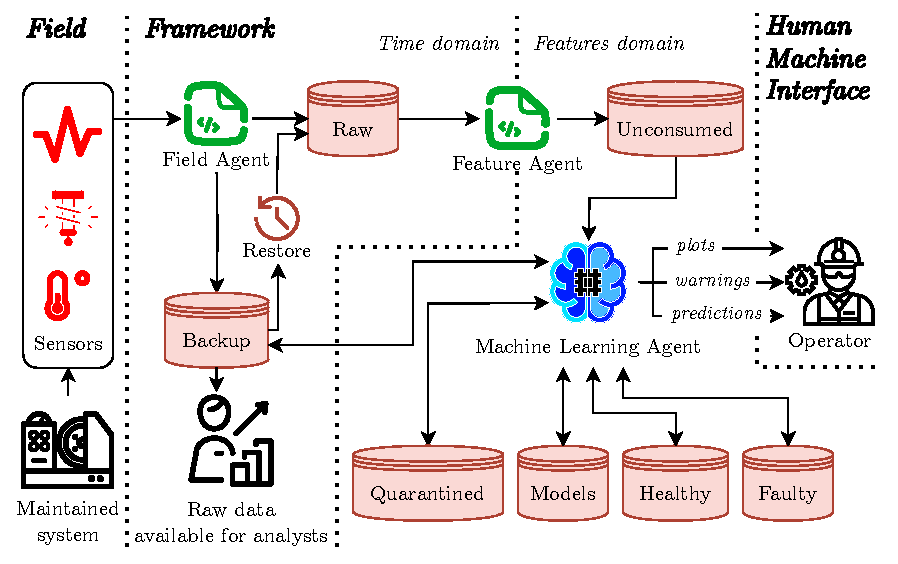
\includegraphics[width=\linewidth]{images/Framework_structure.pdf}
    \caption{The structure of the proposed framework\DIFaddbeginFL \DIFaddFL{. The Field Agent collects the time series, the Feature Agent extracts the features, and the Machine Learning Agent evaluates the health of the maintained device. The agents are connected to collections of a common database.}\DIFaddendFL }
    \label{fig:framework_structure}
\end{figure}

The solution developed in this \DIFdelbegin \DIFdel{project }\DIFdelend \DIFaddbegin \DIFadd{thesis }\DIFaddend is thought to be set up on a new device, and linked to the sensors of the most informative quantities of the system.
In the first phase of commissioning, the framework collects the data, extracts the features and stores them. When the data collected is enough to characterize all the modes of operation of the maintained system, the UML model can be trained. Finally, the framework continues collecting new data, extracting the features, and evaluating the new data. The framework now produces a Novelty Metric (NM) that quantifies how abnormal the new data are. 
This phase can last indefinitely. When the NM overshoots a certain threshold, a warning is issued to the maintenance team. 
\DIFdelbegin \DIFdel{They }\DIFdelend \DIFaddbegin \DIFadd{Then, the team }\DIFaddend can then decide to perform a maintenance action or to continue monitoring the system. If they declare the system as healthy, the framework can be retrained with the new data, to update the UML model. Otherwise, a second UML model can be trained to characterize the newly discovered fault and perform \DIFdelbegin \DIFdel{FD }\DIFdelend \DIFaddbegin \DIFadd{Fault Detection (FD) }\DIFaddend in the future.

\subsection{Software Agents}
The proposed framework is based on software agents. Each agent is autonomous and performs a specific task. The developed agents, as shown in Fig.~\ref{fig:framework_structure}, are:
\begin{itemize}
    \item \textbf{Field Agent (FiA)}: responsible for the synchronous sampling of the data. \DIFaddbegin \DIFadd{It provides the time series records and ensures a correct sampling frequency.
    }\DIFaddend \item \textbf{Feature Agent (FA)}: extracts the features from the time series.
    \item \textbf{Machine Learning Agent (MLA)}: trains the UML algorithms and then performs ND, FD and PM. It reports the results to the user.
\end{itemize}

\subsection{Database}
All the Agents are connected to a common database. In the case of the PC implementation, MongoDB has been used. In the case of the Edge implementation, the data are stored directly in the microcontroller's memory.
Regarding the structure shown in Fig.~\ref{fig:framework_structure}, the MongoDB database is composed of seven collections\DIFdelbegin \DIFdel{: }\emph{\DIFdel{Raw}} %DIFAUXCMD
\DIFdel{containing the time series, }\emph{\DIFdel{Unconsumed}} %DIFAUXCMD
\DIFdel{containing the features to be evaluated by the MLA, }\DIFdelend \DIFaddbegin \DIFadd{. Every collection has a specific role in the framework. For example, the }\DIFaddend \emph{Quarantined, Healthy} and \emph{Faulty} \DIFdelbegin \DIFdel{containing }\DIFdelend \DIFaddbegin \DIFadd{collections contain }\DIFaddend the features that have been flagged as novelty, normal or faulty, respectively, and \emph{Models} \DIFdelbegin \DIFdel{containing }\DIFdelend \DIFaddbegin \DIFadd{contain }\DIFaddend the UML models.
\DIFdelbegin \DIFdel{The collection }\emph{\DIFdel{Backup}} %DIFAUXCMD
\DIFdel{is general purpose.
}\DIFdelend 

\subsection{Multiple Instances}
As shown in Fig.~\ref{fig:multiple_instances}, the framework can be implemented in multiple instances. This is useful to better isolate the location of the anomaly in a complex system. The larger the set of sensors that a single instance of the framework is connected to, the more difficult it is to isolate the anomaly. On the other hand, configuring a large group of sensors allows the detection of complex anomalies.

\begin{figure}
    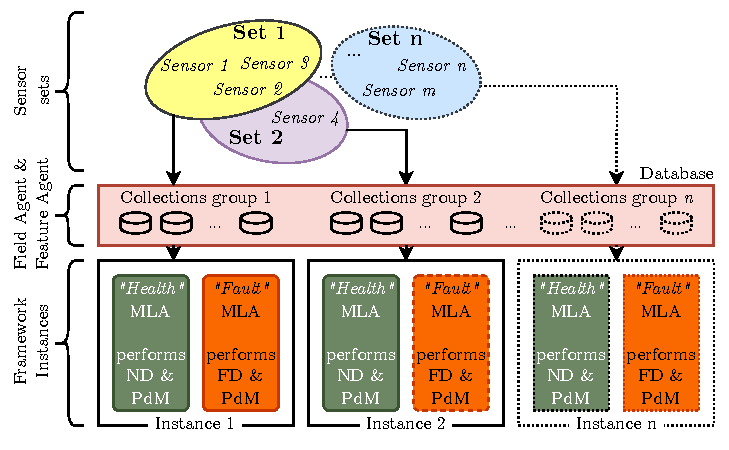
\includegraphics[width=\linewidth]{images/FrameworkInstances.pdf}
    \caption{Multiple instances implementation of the framework\DIFaddbeginFL \DIFaddFL{. Every instance is linked to a different set of sensors, to monitor different parts of the system.}\DIFaddendFL }
    \label{fig:multiple_instances}
\end{figure}


\subsection{Unsupervised Machine Learning Models}

The considered UML implemented in the framework are: \emph{K-means}, \emph{DBSCAN}, \emph{Gaussian Mixture Model} (GMM), \emph{Isolation Forest} (IF), \emph{Local Outlier Factor} (LOF), \emph{One-Class Support Vector Machine} ($\nu$-SVM).

K-means and DBSCAN are traditionally clustering algorithms, so a custom NM has been developed for \DIFdelbegin \DIFdel{this project. In the case of the K-means, the NM is the distance of a new instance in the feature space from the closest centroid, normalized by the cluster radius. For the DBSCAN, the NM is the distance to the new instance from the closest instance in a cluster, normalized by the neighborhood radius.
}%DIFDELCMD < 

%DIFDELCMD < %%%
\DIFdelend \DIFaddbegin \DIFadd{these algorithms. }\DIFaddend The other models are already commonly used for ND, so the NM has been linked to the \quoted{score} provided by the library functions.

If the UML is trained with faulty data to perform FD, the NM measures \quoted{how not faulty} the new data are. In this case, the value is transformed into a Fault Metric (FM) with the function $\text{FM} = - \ln(\text{NM} + 1)$ to preserve the coherence.  \section{FEATURE EXTRACTION}
The framework is developed to acquire time series data from an arbitrary configuration of sensors. \DIFdelbegin \DIFdel{The FiA provides time series records according to a predefined cycle or synchronized with the device operation. It ensures that the sampling process is synchronized with the correct sampling frequency. Once a }\DIFdelend \DIFaddbegin \DIFadd{When a }\DIFaddend time series is available, the FA extracts the features\DIFdelbegin \DIFdel{from the time-domain data}\DIFdelend . Every time series is linked to a specific set of features to be extracted\DIFdelbegin \DIFdel{, configurable in the }\texttt{\DIFdel{.config}} %DIFAUXCMD
\DIFdel{file of the framework}\DIFdelend .

\subsection{Feature set}
The considered features are divided into two categories:
\begin{itemize}
    \item \textbf{Time domain features}: Mean, Standard deviation, Peak-to-peak value (P2P), Root Mean Square value (RMS), Skewness and Kurtosis.
    \item \textbf{Frequency domain features}: Energy of the Wavelet Packet Decomposition (WPD) coefficients, Fast Fourier Transform (FFT) coefficients. The WPD is based on the PyWavelets\footnote{\url{https://github.com/PyWavelets/pywt.git}} \DIFdelbegin \DIFdel{library, for Python, and on the }\DIFdelend \DIFaddbegin \DIFadd{and }\DIFaddend Wavelib\footnote{\url{https://github.com/rafat/wavelib.git}} \DIFdelbegin \DIFdel{library, for C}\DIFdelend \DIFaddbegin \DIFadd{libraries}\DIFaddend .
\end{itemize}

The time domain features are computed in the corrected form for sampled data. In the frequency domain, the WPD is preferred in this work, because it reduces the dimensionality of the feature space. The features are standardized along the training dataset \DIFdelbegin \DIFdel{, }\DIFdelend so that the mean and standard deviation are 0 and 1, respectively. This is done to ease the training of the UML algorithms.

\subsection{Scaling and selection}
\begin{figure}
    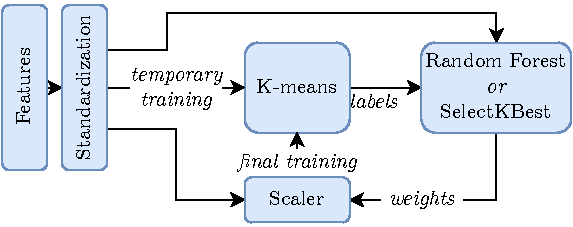
\includegraphics[width=\linewidth]{images/Feat_scaling.pdf}
    \caption{Feature scaling and selection procedure\DIFaddbeginFL \DIFaddFL{. The features are standardized and then scaled by a weight array or selected to reduce the feature space dimensionality, discarding the less informative features.}\DIFaddendFL }
    \label{fig:feature_scaling}
\end{figure}
Despite the standardization, during the experimental validation, it has been observed that some features are more informative than others. To reduce the impact of the less informative features, an optional feature scaling \DIFaddbegin \DIFadd{and selection }\DIFaddend step can be performed\DIFaddbegin \DIFadd{, as shown in Fig.~\ref{fig:feature_scaling}}\DIFaddend . \DIFdelbegin \DIFdel{The scaling is done by multiplying the features by a weight array. }\DIFdelend The weights can be computed by performing a Random Forest training or using the SelectKBest library method. \DIFdelbegin \DIFdel{Alternatively, the weights can be used to remove the less informative features, reducing the dimensionality of the feature space. This procedure is shown in Fig.~\ref{fig:feature_scaling}. }\DIFdelend \section{VALIDATION}
\label{sec:validation}

\subsection{On bearings vibration datasets}

The PC implementation of the framework has been thoroughly tested on a publicly available dataset \DIFdelbegin \DIFdel{provided }\DIFdelend \DIFaddbegin \DIFadd{collected }\DIFaddend by the Center for Intelligent Maintenance Systems (IMS).
The dataset contains time series of \DIFdelbegin \DIFdel{the vibration of four bearings, for a total of }\DIFdelend \DIFaddbegin \DIFadd{vibrations of bearings. It contains }\DIFaddend three separate \quoted{run to failure} experiences. 
\DIFdelbegin \DIFdel{The dataset provides information about the location and type of defects observed after each test.
}\DIFdelend 

\begin{figure}
    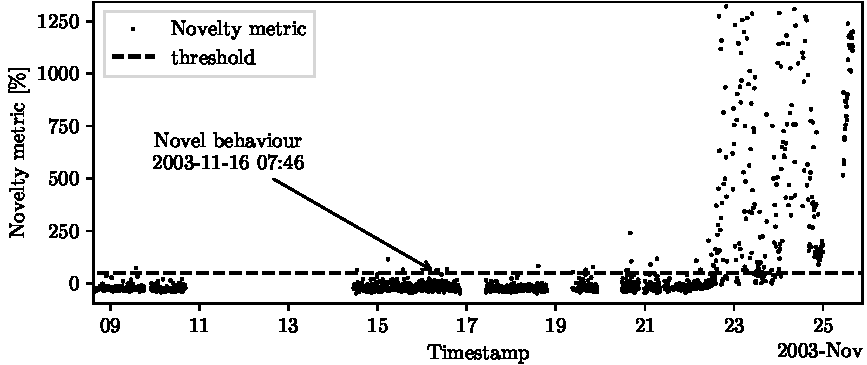
\includegraphics[width=\linewidth]{images/ND_IMS.pdf}
    \caption{Results of ND on the IMS dataset\DIFaddbeginFL \DIFaddFL{. When the Novelty Metric crosses the threshold, a warning is issued. The malfunction happens at the end of the dataset.}\DIFaddendFL }
    \label{fig:ND_IMS}
\end{figure}
\begin{table}
    \centering
    \caption{Comparison of the results for the test n$^\circ$1 of IMS dataset.}
    \label{tab:ims01_comparision}
    \begin{tabular}{lcrr} 
    \toprule
    \textbf{Algorithm} & \textbf{ND event} & \textbf{LT }{[}min] & \textbf{LT }{[}days] \\ 
    \hline
    K-means & 2003-11-16 07:46 & \textbf{13913} & \textbf{9.6} \\
    DBSCAN & 2003-11-22 15:06 & 4833 & 3.3\\
    GMM & 2003-11-22 03:47 & 5513 & 3.8\\
    BGMM & 2003-11-22 03:45 & 5514 & 3.8\\
    $\nu$-SVM & 2003-11-22 14:56 & 4844 &3.3\\
    IF & 2003-11-16 10:08 & 13771 & 9.6\\
    LOF & 2003-11-16 07:48 & 13912 & 9.6\\
    {P2P} without any ML & 2003-11-22 16:06 & 4774 & 3.3\\
    \bottomrule
    \end{tabular}
\end{table}
The ND capability of the framework has been tested using all the \DIFaddbegin \DIFadd{cited }\DIFaddend UML models. The \DIFdelbegin \DIFdel{lead time }\DIFdelend \DIFaddbegin \DIFadd{Lead Time }\DIFaddend (LT) elapsed between the ND event and the actual fault is used to compare the models. The results are compared in table~\ref{tab:ims01_comparision}. The evolution of the NM, using a K-means model on \DIFdelbegin \DIFdel{the "Bearing 3x" }\DIFdelend \DIFaddbegin \DIFadd{a }\DIFaddend signal of the test N$^\circ$1, is shown in Fig.~\ref{fig:ND_IMS}.

\begin{figure}
    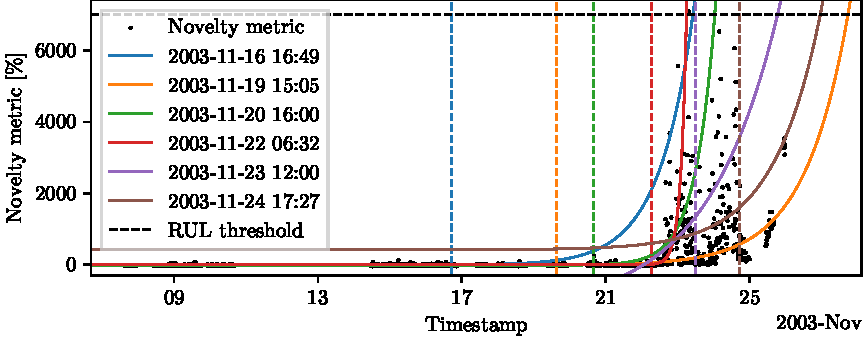
\includegraphics[width=\linewidth]{images/RUL_IMS.pdf}
    \caption{Results of \DIFdelbeginFL \DIFdelFL{RUL }\DIFdelendFL \DIFaddbeginFL \DIFaddFL{Remaining Useful Life }\DIFaddendFL predictions on the IMS dataset\DIFaddbeginFL \DIFaddFL{. The Vertical lines indicate the time when the predictions are performed. The RUL is the time remaining before the fitted curve crosses the threshold.}\DIFaddendFL }
    \label{fig:RUL_IMS}
\end{figure}
To perform PM, the framework has to estimate the Remaining Useful Life (RUL) of the \DIFdelbegin \DIFdel{system}\DIFdelend \DIFaddbegin \DIFadd{component}\DIFaddend . The RUL is predicted \DIFdelbegin \DIFdel{computing when a fitted curve crosses a certain threshold}\DIFdelend \DIFaddbegin \DIFadd{by a curve fitted to the data}\DIFaddend . The type of curve to fit is configurable, in this work $y = a \cdot e^{b \cdot x} + c$ has been used. The results of the RUL predictions are shown in Fig.~\ref{fig:RUL_IMS}.

\begin{figure}
    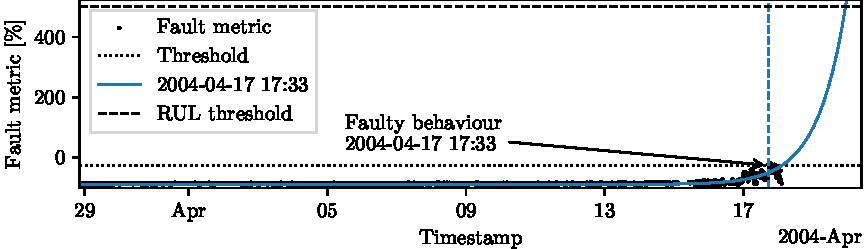
\includegraphics[width=\linewidth]{images/FD_IMS.pdf}
    \caption{Results of FD on the IMS dataset\DIFaddbeginFL \DIFaddFL{. The malfunction is detected when the Fault Metric crosses the threshold. The RUL is the time remaining before the fitted curve crosses the threshold.}\DIFaddendFL }
    \label{fig:FD_IMS}
\end{figure}
Since the second and third tests of the IMS dataset share the same \DIFdelbegin \DIFdel{kind }\DIFdelend \DIFaddbegin \DIFadd{type }\DIFaddend of fault, the framework has been trained to perform FD with the faulty data of the second test and then evaluated on the third. Analogously to the ND, after the FM crosses a certain threshold, a warning is issued and RUL predictions are performed. The results of the FD are shown in Fig.~\ref{fig:FD_IMS}.

\subsection{Laboratory tests}

\begin{figure}
    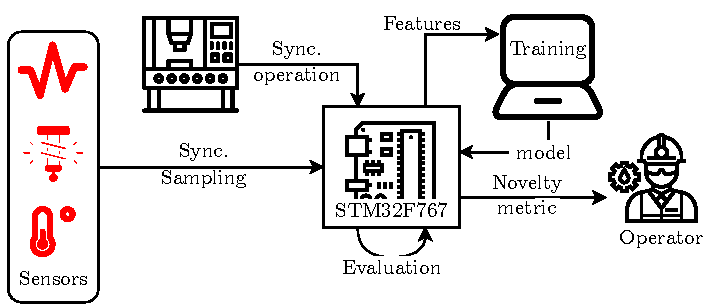
\includegraphics[width=\linewidth]{images/EmbeddedStructure.pdf}
    \caption{Structure of the Edge implementation\DIFaddbeginFL \DIFaddFL{. The microcontroller autonomously evaluates the status of the maintained system. Only during the training phase, the PC implementation computes the model for the Edge.}\DIFaddendFL }
    \label{fig:embedded}
\end{figure}

\DIFdelbegin \DIFdel{Since the validation on the IMS datasethas shown that }\DIFdelend \DIFaddbegin \DIFadd{K-means, IF and LOF are the three models that performed the best on the dataset. K-means performed equally or only slightly better than IF and LOF. Notably, }\DIFaddend the K-means model \DIFdelbegin \DIFdel{is both the simplest and }\DIFdelend \DIFaddbegin \DIFadd{has advantages such as minimal parameter storage requirements and low computational costs for calculating the NM. For these reasons, }\DIFaddend the \DIFdelbegin \DIFdel{most effective, it has been deployed on }\DIFdelend \DIFaddbegin \DIFadd{K-means model has been chosen for }\DIFaddend the Edge implementation.
\DIFaddbegin 

\DIFaddend In the first phase, the framework gathers the data \DIFdelbegin \DIFdel{, }\DIFdelend \DIFaddbegin \DIFadd{and }\DIFaddend extracts the features\DIFdelbegin \DIFdel{and sends them to a PC}\DIFdelend . The UML model is trained on \DIFdelbegin \DIFdel{the }\DIFdelend \DIFaddbegin \DIFadd{a }\DIFaddend PC and then \DIFdelbegin \DIFdel{sent back to }\DIFdelend \DIFaddbegin \DIFadd{included in }\DIFaddend the Edge. After, the microcontroller autonomously evaluates the status of the maintained system. The structure of the Edge implementation is shown in Fig.~\ref{fig:embedded}. 

\begin{figure}
    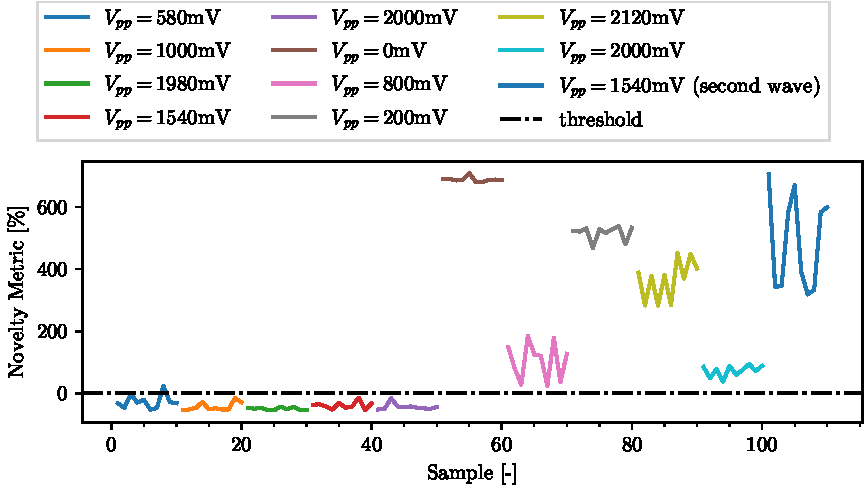
\includegraphics[width=\linewidth]{images/Test02_LOF.pdf}
    \caption{Results of laboratory test on \DIFaddbeginFL \DIFaddFL{the }\DIFaddendFL shaker\DIFaddbeginFL \DIFaddFL{. The first five lines are evaluations of known }\DIFaddendFL vibrations\DIFaddbeginFL \DIFaddFL{, correctly flagged as normal samples. The remaining lines are the successful detections of the novelty of new vibrations.}\DIFaddendFL }
    \label{fig:shaker}
\end{figure}

Extensive tests have been performed on a laboratory shaker, simulating the vibrations generated by a generic mechanical system. The tests have been carried out to evaluate the sensitivity to variations in both amplitude and frequency content\DIFdelbegin \DIFdel{of the vibrations. In Fig.~\ref{fig:shaker} the }\DIFdelend \DIFaddbegin \DIFadd{. The }\DIFaddend results of the ND are shown \DIFaddbegin \DIFadd{in Fig.~\ref{fig:shaker}}\DIFaddend .
\DIFdelbegin \DIFdel{The first five lines are novelty evaluations a repetition of the same signals used for training, and the remaining lines are the successful detections of the novelty.
}\DIFdelend 

A second series of tests has been performed mounting the accelerometer on a linear actuator. The axis of the accelerometer has been aligned with the direction of the movement of the actuator, to sense more the acceleration actuated rather than the vibrations. A set of predefined movement profiles has been used for training, while another set for testing. This series of tests exploited a high number of non-significant features. This is because the WPD gave high resolution on a wide range of frequency content, but the actuator excited only a few, and very low, frequencies. The remaining features were almost all noise, and the standardization procedure had the side effect of amplifying them to the same level as the significant ones. An effort has been made to fine-tune the model to reduce the impact of the noise (see Fig.~\ref{fig:linear}, models 1 to 4). The best result, however, has been obtained by removing the less informative features and using a reduced feature space. The benefit of this approach is evident in Fig.~\ref{fig:linear}\DIFdelbegin \DIFdel{, as \quoted{Model 5} shows a clear and sharp detection of the alternating pattern between known and unknown movement profiles}\DIFdelend .


\begin{figure}
    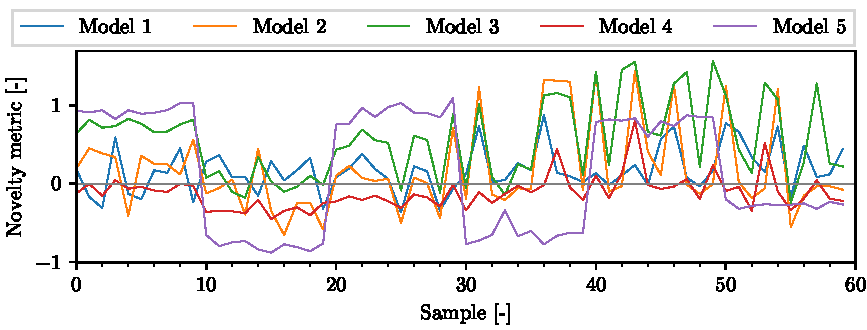
\includegraphics[width=\linewidth]{images/linear.pdf}
    \caption{Results of laboratory test on linear actuator acceleration profiles\DIFaddbeginFL \DIFaddFL{. The dimensionality of the feature space has been reduced to train Model~5, which performs a clear and sharp detection of the alternating pattern between known and unknown movement profiles.}\DIFaddendFL }
    \label{fig:linear}
\end{figure} \section{CONCLUSION AND FUTURE WORK}

The proposed solution has been proven effective in performing Novelty Detection in both public datasets and laboratory tests. The flexibility of the framework allows it to be easily adapted to different systems. 

Some \DIFdelbegin \DIFdel{tests }\DIFdelend \DIFaddbegin \DIFadd{laboratory tests on the Edge implementation }\DIFaddend have shown that the standardization of the features is not always enough to make the clusters in the data space meaningful. In this case, in the PC implementation, Isolation Forest and Local Outlier Factor Models, being not cluster-based, have been tested and resulted as more effective. As future work, the deployment of these models \DIFaddbegin \DIFadd{also }\DIFaddend on the Edge implementation would \DIFdelbegin \DIFdel{bring a significant improvement in }\DIFdelend \DIFaddbegin \DIFadd{improve }\DIFaddend the performance of the framework in some specific applications. 
\end{document}
